\documentclass[12pt,twoside,a4paper,leqno,titlepage]{article}

\makeatletter
\newcommand{\ps@pagenumberfoot}{
\renewcommand{\@oddfoot}{\hfil\thepage}
   \renewcommand{\@evenfoot}{\thepage\hfil}
}
\makeatother

\input{Tyyli.sty}
\pagestyle{pagenumberfoot}
\title{Dokumentaatio}
\author{Tomi Heiskanen}

\begin{document}

\maketitle

\
\thispagestyle{empty}
\newpage

\setcounter{page}{1}
\tableofcontents
\thispagestyle{empty}

\newpage
\section{Johdanto}

Työn aiheena on kurssikysely. Kurssikyselyn avulla kerätään oppilaiden
mielipiteitä ja ideoita kurssin kehittämiseksi. Näiden avulla opettaja voi
kehittää omaa opetusta ja käytettäviä menetelmiä. Oppilaat voivat vastata
kyselyyn nimettömästi.

Työ toteutetaan Helsingin yliopiston tietojenkäsittelytieteen laitoksen users
palvelimella Apache-palvelimen alla. Web-sovelluksen alustajärjestelmän tulee
tukea php-kieltä ja PostgreSQL-tietokantaa.

\section{Käyttötapaukset}

Oppilas haluaa antaa palautetta kurssista ja opetuksesta ja hän voi mennä www-
sivuille ja kertoa sen nimiettömästi. Ohjelma tarkistaa oppilaan statuksen, eli
onko hän kirjoilla opiskelijana ja onko hän kurssilla opiskelijana. Kurssin ulko-
puolinen ei voi antaa palautetta kurssista. Kurssin pitäjä saa lukea palautteet,
mutta hän ei voi yhdistää palautetta kehenkään oppilaaseen. Ulkopuoliset eivät
voi lukea palautteita, mutta on mahdollista saada tietoa palautteiden määrästä
ja voidaan laskea suhde palautteiden määrä/kurssille osallistjat.

\section{Käyttöliittymä}
\begin{figure}[!h]
\centering
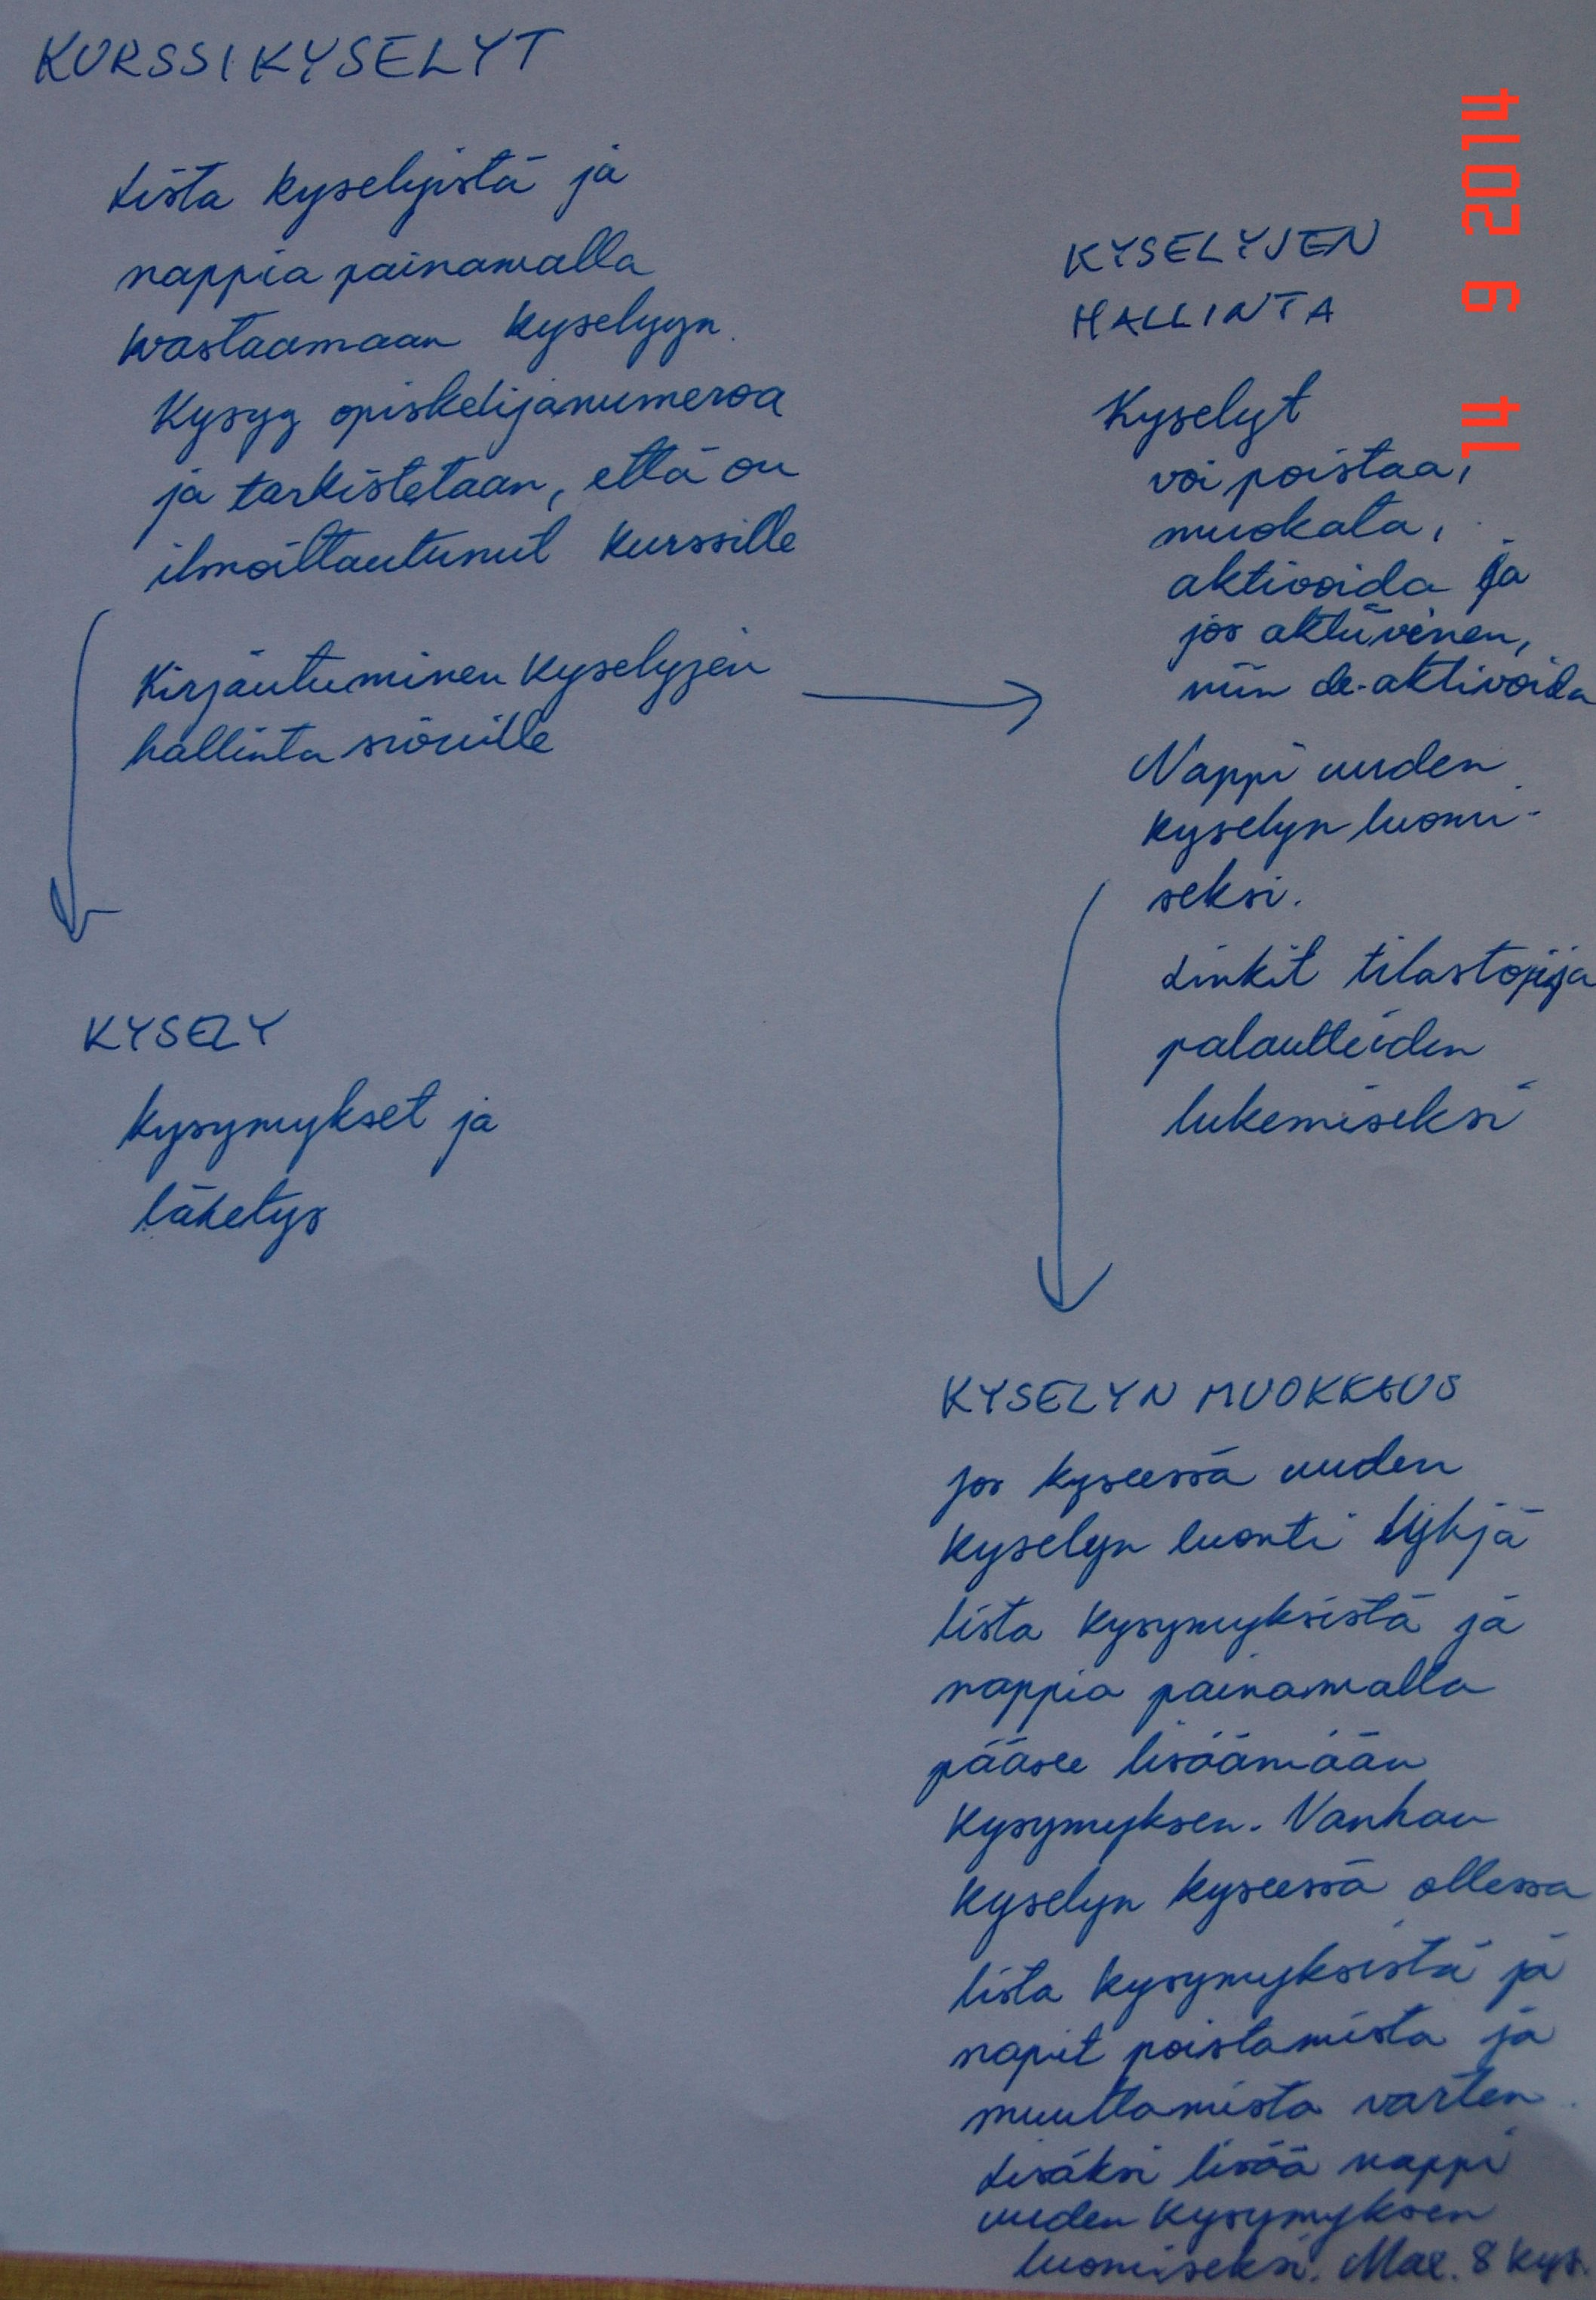
\includegraphics[width=0.7\textwidth]{sivukartta}
\caption{sivukartta}
\end{figure}

\clearpage
\section{Järjestelmän tietosisältö}

\subsubsection*{Kysymykset}

\begin{table}[!h]
\scalebox{0.8}{
\begin{tabular}{|c|c|c|}
  \hline
  % after \\: \hline or \cline{col1-col2} \cline{col3-col4} ...
  \textbf{Attribuutti} & \textbf{Arvojoukko} & \textbf{Kuvailu} \\
  \hline
  KysymysId & Kokonaisluku & Kysymyksen tunnus, joilla kysymykset voidaan
  erottaa \\
  \hline
  kysymys & Merkkijono, max. 150 merkkiä & Kysymys, joka voidaan liittää
  liittää kyselyyn \\
  \hline
\end{tabular}}
\end{table}

\subsubsection*{Opettaja}

\begin{tabular}{|c|c|c|}
  \hline
  % after \\: \hline or \cline{col1-col2} \cline{col3-col4} ...
  \textbf{Attribuutti} & \textbf{Arvojoukko} & \textbf{Kuvailu} \\
  \hline
  OpettajaNro & Kokonaisluku & Identifioi opettajan \\
  \hline
  Etunimi & Merkkijono, max. 20 merkkiä & Opettajan etunimi \\
  \hline
  Sukunimi & Merkkijono, max. 30 merkkiä & Opettajan sukunimi \\
  \hline
\end{tabular}

\subsubsection*{Opiskelija}

\begin{tabular}{|c|c|c|}
  \hline
  % after \\: \hline or \cline{col1-col2} \cline{col3-col4} ...
  \textbf{Attribuutti} & \textbf{Arvojoukko} & \textbf{Kuvailu} \\
  \hline
  OpiskelijaNro & Kokonaisluku & Identifioi opiskelijan \\
  \hline
  Etunimi & Merkkijono, max. 20 merkkiä & Opiskelijan etunimi \\
  \hline
  Sukunimi & Merkkijono, max. 30 merkkiä & Opiskelijan sukunimi \\
  \hline
\end{tabular}

\subsubsection*{Kurssit}

\begin{tabular}{|c|c|c|}
  \hline
  % after \\: \hline or \cline{col1-col2} \cline{col3-col4} ...
  \textbf{Attribuutti} & \textbf{Arvojoukko} & \textbf{Kuvailu} \\
  \hline
  KurssiId & Kokonaisluku & Identifioi kurssin \\
  \hline
  OpettajaNro & Kokonaisluku & Kurssin opettajan opettajanumero \\
  \hline
  KurssinNimi & Merkkijono, max. 40 merkkiä & Kurssin nimi \\
  \hline
\end{tabular}

\subsubsection*{Kurssi-ilmoittautumiset}

\begin{tabular}{|c|c|c|}
  \hline
  % after \\: \hline or \cline{col1-col2} \cline{col3-col4} ...
  \textbf{Attribuutti} & \textbf{Arvojoukko} & \textbf{Kuvailu} \\
  \hline
  KurssiId & Kokonaisluku & Kertoo mikä kurssi on kyseessä \\
  \hline
  OpiskeliNro & Kokonaisluku & Kertoo, kuka opiskelija on ilmoittautunut
  kurssille \\
  \hline
\end{tabular}

\subsubsection*{Kysely}

\begin{tabular}{|c|c|p{5cm}|}
  \hline
  % after \\: \hline or \cline{col1-col2} \cline{col3-col4} ...
  \textbf{Attribuutti} & \textbf{Arvojoukko} & \textbf{Kuvailu} \\
  \hline
  KurssiId & Kokonaisluku & Kertoo, minkä kursssin kurssikysely on \\
  \hline
  Aktiivinen & Merkkijono, max. 5 merkkiä & Kertoo, onko kysely käynnissä vai ei \\
  \hline
\end{tabular}

\section{Relaatiotietokantakaavio}

\begin{figure}[!h]
  \centering
  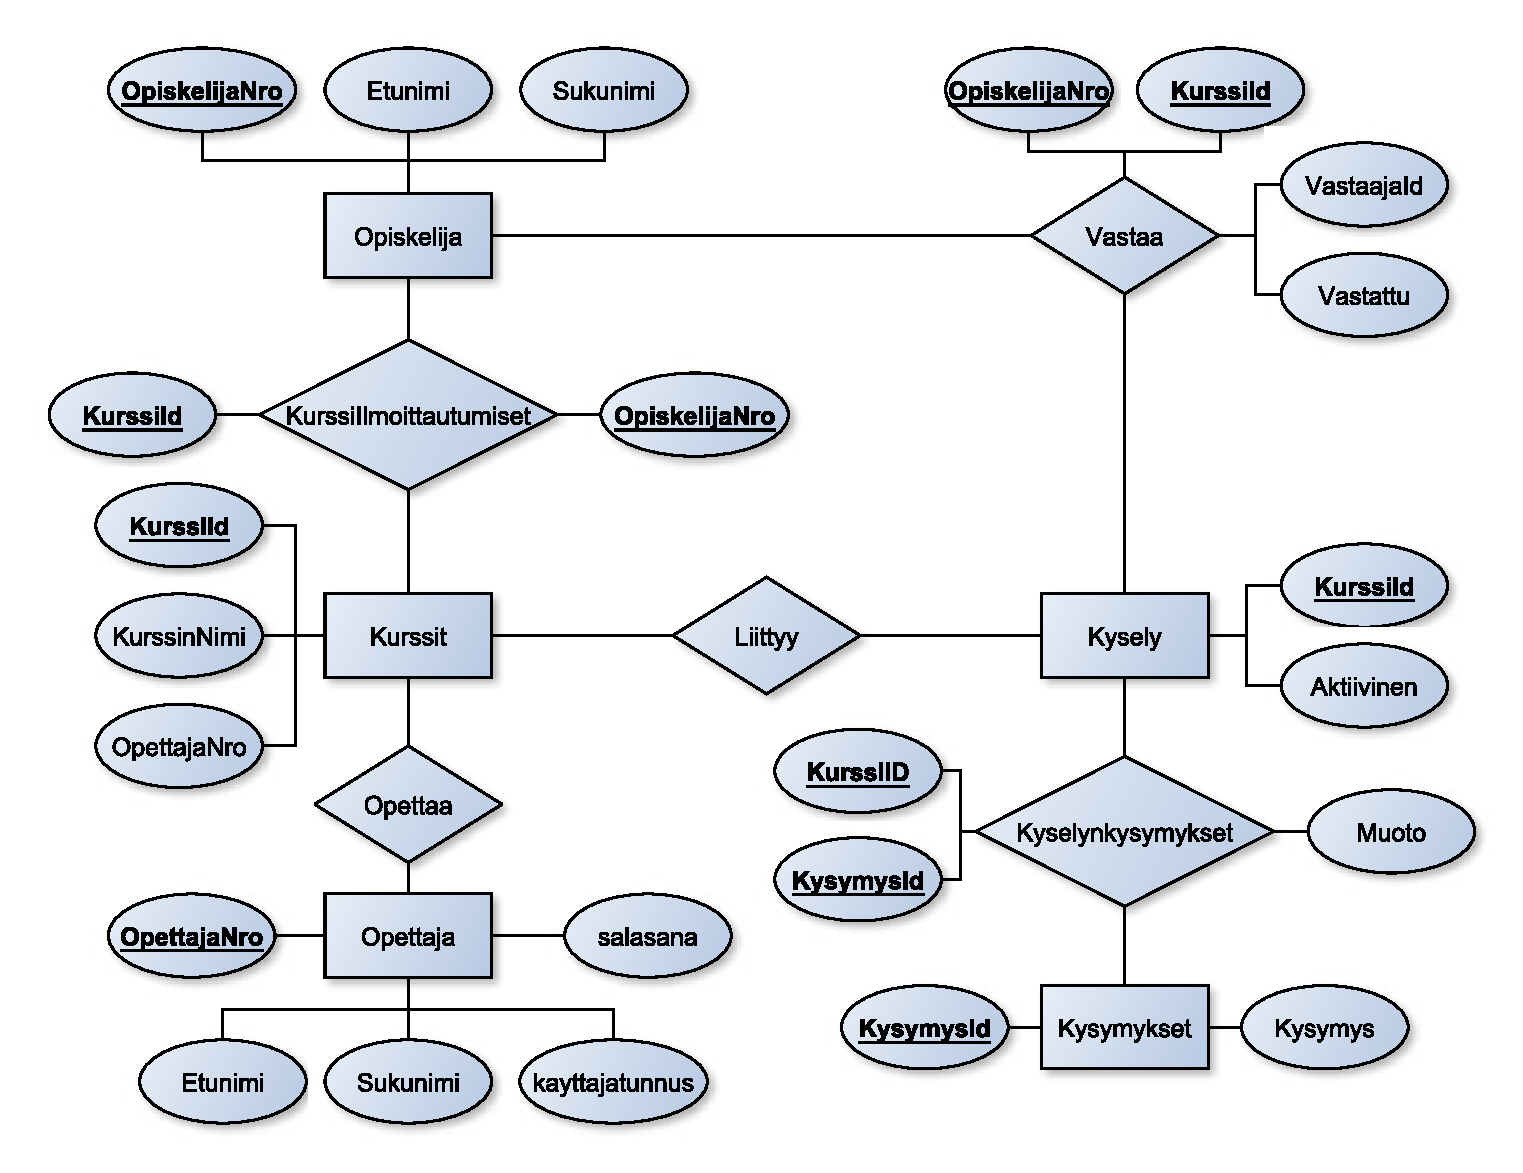
\includegraphics[width=0.9\textwidth]{er-kaavio}\\
  \caption{ER-kaavio}
\end{figure}
\clearpage

\end{document}
